%%%%%%%%%%%%%%%%%%%%%%%%%%%%%%%%%%%%%%%%%%%%%%%%%%%%%%%%%%%%%%%%%%%%%%
%%%%%%%%%%%%%%%%%%%%%%%%%%%%%%%%%%%%%%%%%%%%%%%%%%%%%%%%%%%%%%%%%%%%%%
%%
%% IVT LaTeX template
%%   Joseph Molloy
%%   joseph.molloy@ivt.baug.ethz.ch
%%   
%%   Updates
%%    1.07.2019 | First version of overleaf compatible template for IVT
%%   15.12.1019 | Add german abstract page and fix bug in figure indenting.
%%
%%%%%%%%%%%%%%%%%%%%%%%%%%%%%%%%%%%%%%%%%%%%%%%%%%%%%%%%%%%%%%%%%%%%%%
%%%%%%%%%%%%%%%%%%%%%%%%%%%%%%%%%%%%%%%%%%%%%%%%%%%%%%%%%%%%%%%%%%%%%%

%%%%%%%%%%%%%%%%%%%%%%%%%%%%%%%%%%%%%%%%%%%%%%%%%%%%%%%%%%%%%%%%%%%%%%
%%%%%%%%%%%%%%%%%%%%%%%%%%%%%%%%%%%%%%%%%%%%%%%%%%%%%%%%%%%%%%%%%%%%%%
%%
%% This is an example for writing a paper at the IVT.
%% It supports English and German language.
%% By using it, it is possible to switch paper layouts easily
%% (e.g., working paper style into TRB style)
%%
%% Include german option in document class for german headings (i.e. Literatur)
%% \documentclass[numbered, german]{ivt-style/standard}
%%%%%%%%%%%%%%%%%%%%%%%%%%%%%%%%%%%%%%%%%%%%%%%%%%%%%%%%%%%%%%%%%%%%%%
%%%%%%%%%%%%%%%%%%%%%%%%%%%%%%%%%%%%%%%%%%%%%%%%%%%%%%%%%%%%%%%%%%%%%%
%%%%%%%
\documentclass[numbered]{ivt-style/standard}
%\documentclass{ivt-style/trb}

\RequirePackage[capitalize]{cleveref}
\RequirePackage{booktabs}

\providecommand{\ivthline}{}

\title{The title of the paper}
\subtitle{Do you really need a subtitle?}
\papertype{The type of paper}

\headingstitle{A Short title for the header}


\author{
  Joseph Molloy \\
  IVT \\
  ETH Zürich \\
  CH-8093 Zurich \\
  \texttt{joseph.molloy@ivt.baug.ethz.ch}
  \and
  Second Author \\
  IVT \\
  ETH Zurich
  \and
  Third Author \\
  IVT \\
  ETH Zurich
  \and
  Fourth Author \\
  IVT \\
  ETH Zurich
}

\reportdate{December 2019}
\reportdategerman{Dezember 2019}
\reportnumber{10XX}
\titlefigure{figures/MATSimLoop}
% The year of the paper
% The month of the paper, include only: jan,feb,mar,apr,may,jun,jul,aug,sep,oct,nov,dec
% The day of the paper - include day in number 1,..., 12,..., 31


%%%% If you don't want to include an english abstract page, comment out this command
\abstract{
    Lorem ipsum dolor sit amet, consectetur adipiscing elit, sed do eiusmod tempor incididunt ut labore et dolore magna aliqua. Ut enim ad minim veniam, quis nostrud exercitation ullamco laboris nisi ut liquip ex ea commodo consequat. Duis aute irure dolor in reprehenderit in voluptate velit esse cillum dolore eu fugiat nulla pariatur. Excepteur sint occaecat cupidatat non proident, sunt in culpa qui officia deserunt mollit anim id est laborum.
 }

%%% To inclue a second abstract page with german headings and a german abstract, use the command below
\germanabstract{
    Dieses Bericht....

}

\keywords{keyword1, keyword2, etc}

\suggestedCitation{Fill in the suggested citation format for your paper here}

\begin{document}
\maketitle
\clearpage
%start the paper/report here

%\clearpage
%\tableofcontents
%\clearpage
%\listoffigures
%\listoftables
%\clearpage

\tableofcontents
\listoftables
\listoffigures
\newpage

%%%%%%%%%%%%%%%%%%%%%%%%%%%%%%%%%%%%%%%%%%%%%%%%%%%%%%%%%%%%%%%%%%%%%%
%
\section{Introduction}
%
%%%%%%%%%%%%%%%%%%%%%%%%%%%%%%%%%%%%%%%%%%%%%%%%%%%%%%%%%%%%%%%%%%%%%%

This is a small overview how to write papers at the IVT in \LaTeX.

If you see bugs and errors in the layout please contact
joseph.molloy@ivt.baug.ethz.ch.

%%%%%%%%%%%%%%%%%%%%%%%%%%%%%%%%%%%%%%%%%%%%%%%%%%%%%%%%%%%%%%%%%%%%%%
\subsection{Structuring}
%%%%%%%%%%%%%%%%%%%%%%%%%%%%%%%%%%%%%%%%%%%%%%%%%%%%%%%%%%%%%%%%%%%%%%

To structure you paper you can define several headings and
subheadings:
``\textbackslash{}section'', ``\textbackslash{}subsection'',
``\textbackslash{}subsubsection'', ``\textbackslash{}paragraph'' and
``\textbackslash{}subparagraph''. The first three will be numbered and
will show
up in the content. The layout defines the style of the headings.

Examples of sections and subsections:

\subsubsection{A subsubsection}

Some text. Some text. Some text. Some text. Some text. Some text. Some
text. Some text. Some text. Some text. Some text. Some text. Some
text. Some text. Some text. Some text.

\paragraph{A paragraph}

Some text. Some text. Some text. Some text. Some text. Some text. Some
text. Some text. Some text. Some text. Some text. Some text. Some
text. Some text. Some text. Some text.

\subparagraph{A subparagraph}

Some text. Some text. Some text. Some text. Some text. Some text. Some
text. Some text. Some text. Some text. Some text. Some text. Some
text. Some text. Some text. Some text.

\subsection{A Really Really Really Really Really Really Really Really Really Really Really Really Long Section title}
%%%%%%%%%%%%%%%%%%%%%%%%%%%%%%%%%%%%%%%%%%%%%%%%%%%%%%%%%%%%%%%%%%%%%%
\subsubsection{Page Break}
%%%%%%%%%%%%%%%%%%%%%%%%%%%%%%%%%%%%%%%%%%%%%%%%%%%%%%%%%%%%%%%%%%%%%%

There are three ways of performing a manual page break.
\begin{itemize}
  \item ``\textbackslash{}clearpage'': omits the remaining space of the
current page and starts the new one. Inserting two or more times that
command does NOT produce follow up empty pages.
  \item ``\textbackslash{}cleardoublepage'': It does the same than the
command above, but for a report \LaTeX\ type that define different
layouts for the odd and even pages (i.e.\ dissertation layouts), it
sometimes produces a complete follow up empty page such that the next
sections will occur always on the even page (odd page, resp.)
  \item ``\textbackslash{}include'': This is another way to start on a
new page. If you use the ``\textbackslash{}include''
command for separating a paper
into different \texttt{.tex} files,
``\textbackslash{}include'' will always start on
top of the next page. If you do not want that, but still want to
separate the paper into different files,
use the ``\textbackslash{}input''
command instead.
\end{itemize}

\clearpage

\cleardoublepage

%%%%%%%%%%%%%%%%%%%%%%%%%%%%%%%%%%%%%%%%%%%%%%%%%%%%%%%%%%%%%%%%%%%%%%
\subsection{Text Blocks}
%%%%%%%%%%%%%%%%%%%%%%%%%%%%%%%%%%%%%%%%%%%%%%%%%%%%%%%%%%%%%%%%%%%%%%

A newline (one time ``Return'') does NOT produce a new Block.
You have to separate blocks with a COMPLETE EMPTY line.

Hence, it is a good idea to insert hard line breaks frequently,
e.g.~after commas or full stops.
Most version control systems such as SVN are line-based;
changes can be tracked easier if a paragraph is split
over several lines.
By the same token, it is not a good idea to let your text editor
manage the line breaks for you.

This is a block. This is a block. This is a block. This is a block.
This is a block. This is a block. This is a block. This is a block.
This is a block. This is a block. This is a block. This is a block.
This is a block. This is a block. This is a block.

This is another block. This is another block. This is another block.
This is another block. This is another block. This is another block.
This is another block. This is another block. This is another block.
This is another block. This is another block. This is another block.
This is another block. This is another block. This is another block.

%%%%%%%%%%%%%%%%%%%%%%%%%%%%%%%%%%%%%%%%%%%%%%%%%%%%%%%%%%%%%%%%%%%%%%
\subsection{Lists}
%%%%%%%%%%%%%%%%%%%%%%%%%%%%%%%%%%%%%%%%%%%%%%%%%%%%%%%%%%%%%%%%%%%%%%

There are three ways of making lists:

\subsubsection{Items}

\begin{itemize}
  \item Item one
  \begin{itemize}
    \item Item one
    \item Item two Item two Item two Item two Item two Item two Item
    two Item two
    Item two Item two Item two Item two Item two Item two Item
    two Item two
    \item Item three
  \end{itemize}
  \item Item two Item two Item two Item two Item two Item two Item two
Item twoItem two Item two Item two Item two Item two Item two Item two
Item two
  \item Item three
\end{itemize}

\subsubsection{Enumerations}

\begin{enumerate}
  \item Item one
  \begin{enumerate}
    \item Item one
    \item Item two Item two Item two Item two Item two Item two Item
two Item twoItem two Item two Item two Item two Item two Item two Item
two Item two
    \item Item three
  \end{enumerate}
  \item Item two Item two Item two Item two Item two Item two Item two
Item twoItem two Item two Item two Item two Item two Item two Item two
Item two
  \item Item three
\end{enumerate}

\subsubsection{Descriptive list}

\begin{description}
  \item[Desc one] Item one
  \begin{description}
    \item[Desc one] Item one
    \item[Desc two] Item two Item two Item two Item two Item two Item
two Item two Item two Item two Item two Item two Item two Item two
Item two Item two Item two Item two
    \item[Desc three] Item three
  \end{description}
  \item[Desc two] Item two Item two Item two Item two Item two Item
two Item two Item two Item two Item two Item two Item two Item two
Item two Item two Item two Item two
  \item[Desc three] Item three
\end{description}

\subsubsection{Sub-Lists}

List can be nested in any fashion you like:

\begin{itemize}
  \item Item one
  \begin{itemize}
    \item Item one
    \item Item two
    \item Item three
  \end{itemize}
  \item Item three
  \begin{enumerate}
    \item Item one
    \begin{description}
      \item[Desc one] Item one
      \item[Desc two] Item two Item two Item two Item two Item two
Item two Item two Item two Item two Item two Item two Item two Item
two Item two Item two Item two Item two
      \begin{itemize}
        \item Item one
        \item Item two Item two Item two Item two Item two Item
        two Item two Item two Item two Item two Item two Item two
        Item two Item
        two Item two Item two Item twoItem two
        \item Item three
      \end{itemize}
      \item[Desc three] Item three
      \begin{enumerate}
        \item Item one
        \item Item two Item two Item two Item two Item two Item two
        Item two Item two Item two Item two Item two Item two
        Item two Item
        two Item two Item two Item two Item two Item two Item two Item two Item
        two
        \item Item three
      \end{enumerate}
    \end{description}
    \item Item two
    \item Item three
  \end{enumerate}
  \item Item four
\end{itemize}

%%%%%%%%%%%%%%%%%%%%%%%%%%%%%%%%%%%%%%%%%%%%%%%%%%%%%%%%%%%%%%%%%%%%%%
\subsection{Text appearance}
%%%%%%%%%%%%%%%%%%%%%%%%%%%%%%%%%%%%%%%%%%%%%%%%%%%%%%%%%%%%%%%%%%%%%%

There are also more commands to change the appearance of text.
However, underlining and letter-spacing
is not recommended when writing papers.
Some even consider bold-face as bad practice, as it changes
the ``average greyness'' of the text
(as does underlining and letter-spacing).

\subsubsection{Bold, etc.}

\emph{Emphasis (instead of italic)}, \textbf{Bold},
\textsc{Small caps}, \textbf{\textit{Bold italics}},
\texttt{Teletype}, \textsf{Sans serif}.

\subsubsection{URL}

To write an url type: \url{www.ivt.ethz.ch}.
The PDF will contain a link to that URL.

%%%%%%%%%%%%%%%%%%%%%%%%%%%%%%%%%%%%%%%%%%%%%%%%%%%%%%%%%%%%%%%%%%%%%%
\subsection{Special Characters}
%%%%%%%%%%%%%%%%%%%%%%%%%%%%%%%%%%%%%%%%%%%%%%%%%%%%%%%%%%%%%%%%%%%%%%

\subsubsection{Large Space}

Two sentence are separated with a large empty space. For dots used in
acronyms (``i.e.'' or ``e.g.'') followed by an empty space, you do not
want this extra large space. In this case you should add a backslash
after the dot
or use non-breaking space (see below).
Example:

A fact, e.g.\ an example.

\subsubsection{Quotation Mark}

Quotation marks: ``text to be quoted'', also in `single quotes'.

\subsubsection{Dashes}

There are three types of dashes:
\begin{description}
  \item[Hyphen Dash] agent-based
  \item[Range Dash] page 123--138
  \item[em Dash] bla bla---thinking---bla bla
\end{description}

\subsubsection{Predefined special characters}

Some characters are used for special functions. If you want to write
them use the following substitutions:

\$
\&
\%
\#
\{
\}
%
\S{}
\pounds{}
\textbackslash{}
\textasciitilde{}
\textasciicircum{}
%
?`
!`

There are a lot more special characters, especially for formulas.
You will find a fairly good overview in
\href{http://www.ctan.org/tex-archive/info/lshort/english/lshort.pdf}{\texttt{lshort.pdf}}.
This is by the way a good reference for many questions concerning \LaTeX{}.

\subsubsection{Non-breaking space}

Sometimes, you do not want that two words are split at a line ending.
To prevent this use the ``tilde'' character. Example:

6~AM 6~AM 6~AM 6~AM 6~AM 6~AM 6~AM 6~AM 6~AM 6~AM 6~AM 6~AM 6~AM 6~AM
6~AM 6~AM

versus

6 AM 6 AM 6 AM 6 AM 6 AM 6 AM 6 AM 6 AM 6 AM 6 AM 6 AM 6 AM 6 AM 6 AM
6 AM 6 AM

\subsubsection{Ligatures}

Take a closer look at the words ``affluent'', ``effective'' and ``flow''.
The joining of the f and l letters
happens automatically; however on rare occasions
you may want to
suppress this, like for ``shelf{}ful''.

%%%%%%%%%%%%%%%%%%%%%%%%%%%%%%%%%%%%%%%%%%%%%%%%%%%%%%%%%%%%%%%%%%%%%%
%
\section{Complex Structures}
%
%%%%%%%%%%%%%%%%%%%%%%%%%%%%%%%%%%%%%%%%%%%%%%%%%%%%%%%%%%%%%%%%%%%%%%

Here you can find how to use labeling, cross-references, footnotes,
etc. Some of them are standard \LaTeX\ commands,
described in this section.
Commands available only in the IVT environment
will be explained in the next section.

%%%%%%%%%%%%%%%%%%%%%%%%%%%%%%%%%%%%%%%%%%%%%%%%%%%%%%%%%%%%%%%%%%%%%%
\subsection{Labels and Cross-Refs}
\label{sec:compStructs-LabelsCrossRefs}
%%%%%%%%%%%%%%%%%%%%%%%%%%%%%%%%%%%%%%%%%%%%%%%%%%%%%%%%%%%%%%%%%%%%%%

Anywhere you want you can add a label (see above for this subsection).
Wherever you want you can refer (cross-ref) to this label by using the
``\textbackslash{}ref'' command.
Example:
Labels and Cross-Refs can be found in
\cref{sec:compStructs-LabelsCrossRefs}.

Labels can also be used in lists:

\begin{enumerate}
  \item\label{item:stepOne} Step one
  \item Step two
  \item Feedback (Goto~\ref{item:stepOne})
\end{enumerate}

Labels are very important in Figures and Tables. It is used to refer
to them
in the written text (see \cref{sec:compStructs-Figures,sec:compStructs-Tables}).

%%%%%%%%%%%%%%%%%%%%%%%%%%%%%%%%%%%%%%%%%%%%%%%%%%%%%%%%%%%%%%%%%%%%%%
\subsection{Clever referencing}\label{sec:CleverReferencing}
%%%%%%%%%%%%%%%%%%%%%%%%%%%%%%%%%%%%%%%%%%%%%%%%%%%%%%%%%%%%%%%%%%%%%%

The ``cleveref'' package provides the ``\textbackslash{}cref'' command to conveniently
reference any type of object\footnote{See
\href{http://www.ctan.org/tex-archive/help/Catalogue/entries/cleveref.html}{its CTAN entry},
accessed on May 28th, 2010.}. For example:

\begin{itemize}
  \item This is a reference to a single section: Labels are described
in \cref{sec:compStructs-LabelsCrossRefs}.
  \item This is a reference to multiple sections: This document
contains, among others,
\cref{sec:compStructs-LabelsCrossRefs,sec:footnotes,sec:CleverReferencing}.
  \item This is a reference to multiple subsequent sections: This
document contains, among others,
\cref{sec:compStructs-LabelsCrossRefs,sec:footnotes,sec:compStructs-Figures}.
  \item One can summarize refs to different types of objects. This
becomes clear when taking a look at this sentence with references to
\cref{sec:compStructs-LabelsCrossRefs,tab:labelOfTheTable}.
  \item \Cref{fig:labelOfTheSingleFigure}---this is how a reference to a figure
    should look like at the beginning of a sentence.
\end{itemize}

Note how ``cleveref'' automatically adds the object type. One does not
have to write it anymore.
But remember using the ``\textbackslash{}Cref'' command instead
at the beginning of the sentence!

%%%%%%%%%%%%%%%%%%%%%%%%%%%%%%%%%%%%%%%%%%%%%%%%%%%%%%%%%%%%%%%%%%%%%%
\subsection{Footnotes}\label{sec:footnotes}
%%%%%%%%%%%%%%%%%%%%%%%%%%%%%%%%%%%%%%%%%%%%%%%%%%%%%%%%%%%%%%%%%%%%%%

Footnotes are directly embedded in the text where you want to refer to
them.
Depending on the layout, they will appear at the bottom of the current
page or
at the end of the Section. Example:

This is a text\footnote{more information about ``text''} with a
footnote\footnote{more information about ``footnote''}.


%%%%%%%%%%%%%%%%%%%%%%%%%%%%%%%%%%%%%%%%%%%%%%%%%%%%%%%%%%%%%%%%%%%%%%
\subsection{Formulas}
%%%%%%%%%%%%%%%%%%%%%%%%%%%%%%%%%%%%%%%%%%%%%%%%%%%%%%%%%%%%%%%%%%%%%%

To write formulas in \LaTeX{} you can describe it as plain text.
You can either embed a formula into the text or add it on a separate
line.
In the second version formula numbers will be automatically added.
With labels you are able to refer to the formulas.

\subsubsection{Formula embedded in text}

The formula part is enclosed by \$. Examples:

bla bla bla $[-30min,+30min]$ bla bla bla.

bla bla bla bla bla bla $P > N$ bla bla bla $S_{j}$ bla $j$ bla bla
bla  $\beta$ bla bla bla.

\subsubsection{Formula as separate line}

Using the ``linenomath'' and ``flalign'' environments the formulas will be placed on a
separate line with a number. Examples:

\begin{linenomath}
  \begin{flalign}
  \label{eq:score-averaging}
  S = (1 - \alpha) \cdot S_\text{old} + \alpha \cdot S_\text{new}
  \end{flalign}
\end{linenomath}

\begin{linenomath}
  \begin{flalign}
  \label{eq:utility-total}
  U_\text{total} = \sum_{i=1}^{n} U_{\text{perf},i} + \sum_{i=1}^{n} U_{\text{late},i}
              + \sum_{i=1}^{n} U_{\text{travel},i}\,,
   \end{flalign} 
\end{linenomath}

\begin{linenomath}   
    \begin{flalign}   
    \label{eq:utility-perform}
  U_{\text{perf},i}(t_{\text{perf},i}) = \max \left[ 0 , \beta_{\text{perf}} \cdot
t^{*}_{i} \cdot
                \ln \left( \frac{t_{\text{perf},i}}{t_{0,i}} \right)
\right]\,,
   \end{flalign} 
\end{linenomath}

\begin{linenomath}   
    \begin{flalign}   
    \label{eq:typical-duration}
  t_{0,i} = t^{*}_{i} \cdot e^{-\zeta / (p \cdot t^{*}_i)}\,,
   \end{flalign} 
\end{linenomath}

\begin{linenomath}   
    \begin{flalign}   
    \label{eq:utility-perform-resolved}
  U_{\text{perf},i}(t_{\text{perf},i}) = 
      \max\left[ 0 , \beta_\text{perf} \cdot t^{*}_{i} \cdot
      \left( \ln\left( \frac{t_{\text{perf},i}}{t^{*}_{i}} \right) +
      \frac{\zeta}{p \cdot t^{*}_i} \right) \right].
   \end{flalign} 
  \end{linenomath}

\begin{linenomath}   
    \begin{flalign}   
    \label{eq:utility-late}
  U_{\text{late},i} = \begin{cases} 
    \beta_{\text{late}} \cdot t_{\text{late},i}
      &: t_{\text{late},i} \geq 0 \\
    0
      &: \text{otherwise}
  \end{cases}
   \end{flalign} 
 \end{linenomath}

\begin{linenomath}   
    \begin{flalign}   
    \label{eq:utility-travel}
  \begin{aligned}
    U_{\text{travel},i} &= \beta_{\text{travel}} \cdot t_{\text{travel},i} \\
                        &= \beta_{\text{travel}} \cdot \ldots
  \end{aligned}
   \end{flalign} 
\end{linenomath}

With the labels you can refer to an equation with the ``ref'' command.
Examples:

As shown in \cref{eq:utility-total}, the total utility is\ldots{}
See \cref{eq:utility-travel} for the definition of the
travel-utility.

\subsubsection{Text mode}

Text in math mode looks ugly, and spaces are ignored:
$bafflingly ugly$.
Anything that consists of more than one letter
should be surrounded by the ``\textbackslash{}text'' command:
$\text{bafflingly ugly}$.
If you need italics, use ``\textbackslash{}text\{\textbackslash{}emph\{\ldots\}\}''
or simply
 ``\textbackslash{}mathit'';
the latter still eats spaces:
$\mathit{bafflingly ugly}$.

%%%%%%%%%%%%%%%%%%%%%%%%%%%%%%%%%%%%%%%%%%%%%%%%%%%%%%%%%%%%%%%%%%%%%%
\subsection{Citations and References}
%%%%%%%%%%%%%%%%%%%%%%%%%%%%%%%%%%%%%%%%%%%%%%%%%%%%%%%%%%%%%%%%%%%%%%

By using the IVT bibliography database you can refer to a reference by
using the command ``\textbackslash{}citep'' (citation in parentheses)
or ``\textbackslash{}citet''
(citation embedded in the sentence). With the unique key of the
bib-entry you will automatically refer to that reference and the
reference will automatically be added to the reference list. The way
the references will be sorted depends on the layout you use. 

Examples for ``\textbackslash{}citet'':

bla bla \citet{axhausen2008income} and
\citet{matsimbook}
bla bla bla bla bla bla bla bla bla bla
\citet{axhausen2008income,matsimbook}
bla bla bla bla bla bla bla bla.

Examples for ``\textbackslash{}citep'':

bla bla bla bla bla bla
\citep[e.g.,]{matsimbook,axhausen2008income}.

bla bla bla bla bla bla \citep[see also][pp.325-378]{axhausen2008income}.

bla bla bla bla bla bla \citep{axhausen2008income}.

Just like with the clever referencing commands (cf.~\cref{sec:CleverReferencing})
you should use ``\textbackslash{}Citet'' or ``\textbackslash{}Citep'' instead
at the beginning of a sentence.
\Citet{axhausen2008income}
would be otherwise shown as \citet{axhausen2008income}
in your paper.

%%%%%%%%%%%%%%%%%%%%%%%%%%%%%%%%%%%%%%%%%%%%%%%%%%%%%%%%%%%%%%%%%%%%%%
%
\section{Figures and Tables}
%
%%%%%%%%%%%%%%%%%%%%%%%%%%%%%%%%%%%%%%%%%%%%%%%%%%%%%%%%%%%%%%%%%%%%%%

This section defines the
special commands that are available only at the IVT environment.
Those special commands
react on different layouts defined in the environment,
thus making it convenient to switch between paper layouts.

%%%%%%%%%%%%%%%%%%%%%%%%%%%%%%%%%%%%%%%%%%%%%%%%%%%%%%%%%%%%%%%%%%%%%%
\subsection{Figures} \label{sec:compStructs-Figures}
%%%%%%%%%%%%%%%%%%%%%%%%%%%%%%%%%%%%%%%%%%%%%%%%%%%%%%%%%%%%%%%%%%%%%%

There are three commands for including Figures. One for a single Figure
and one for a Multi-Figure. The position of the Figure is chosen by
\LaTeX,
but a hint can be provided.

\subsubsection{Single Figures}

\label{sec:compStructs-Figures-SingleFigures}

A single figure as shown in \cref{fig:labelOfTheSingleFigure}
has the following construct:

\textbackslash{}begin[placement]\{figure\} as in normal latex 

The placement modifier 
specifies where the figure appears in the final document.
It can be ``tp'', ``htp'' or ``hp'';
``t'' means ``at the top of this or a following page'',
``h'' means ``at the place where the command appears'',
and ``p'' means ``on a separate page''.
If you leave out this parameter (including the square brackets),
``tp'' is the default.
Usually a figure will appear on the next suitable location
after it has been declared.
The placement on a separate page will be used as a last resort
if the figure does not fit anywhere else, even if you do not include it.

With \textbackslash{}ivtsource\{text\} you can add a source. If you do not want
to add a source, just leave it empty. If not, ``Source: '' or
``Quelle: '' will be added followed by your text.


%---------------------------------------------------------------------
\begin{figure}%
\caption{Single Figure: Here you can add the long Caption of the Figure.}%
\label{fig:labelOfTheSingleFigure}%
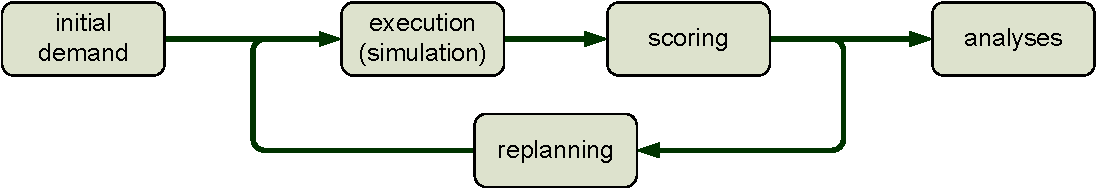
\includegraphics[width=1.0\textwidth]{figures/MATSimLoop}%
\ivtsource{Christoph Dobler}
\ivthline
\end{figure}

%%%%%%%%%%%%%%%%%%%%%%%%%%%%%%%%%%%%%%%%%%%%%%%%%%%%%%%%%%%%%%%%%%%%%%
\subsection{Tables} \label{sec:compStructs-Tables}
%%%%%%%%%%%%%%%%%%%%%%%%%%%%%%%%%%%%%%%%%%%%%%%%%%%%%%%%%%%%%%%%%%%%%%

A table has the same structure as the single Figure (see above). But
instead of including a graphic in item~4 you add the ``tabular''
construct.
Unfortunately it is not that easy to understand and edit such a table. One has
to get used to it. 
However, quite a few tools can help converting the data
to the \LaTeX{} format,
see \url{http://tex.stackexchange.com/q/49414/8057}
for an overview.

If you do not like it you can still add the table
as a graphic (with the ``\textbackslash{}includegraphics'') command.
But you still need
to use the ``\textbackslash{}createtable'' command,
otherwise your table will appear
in the list of figures instead of the list of tables.
\Cref{tab:labelOfTheTable} shows an example of a table.

%---------------------------------------------------------------------
\begin{table}[!ht]
\caption{A Tables  Caption}
\label{tab:labelOfTheTable}%

\begin{tabular}[c]{lr@{.}lcr@{.}l}
    \toprule
    Bias / Error     & \multicolumn{2}{c}{Routes Only} &
\multicolumn{3}{c}{Times and Routes} \\
    \midrule
    Mean Abs. Bias:  & $+$331&40                        && $+$306&32  
                         \\
    Mean Rel. Bias:  &  $+$19&62\%                      &&  $+$25&27\%
                         \\
    \midrule
    Mean Abs. Error: &    533&55                        &&    503&77  
                         \\
    Mean Rel. Error: &     37&50\%                      &&     35&38\%
                         \\
    \bottomrule
  \end{tabular}

\ivtsource{my source}
\ivthline
\end{table}
%---------------------------------------------------------------------



%%%%%%%%%%%%%%%%%%%%%%%%%%%%%%%%%%%%%%%%%%%%%%%%%%%%%%%%%%%%%%%%%%%%%%
%
\section{Summary and Important Notes}
%
%%%%%%%%%%%%%%%%%%%%%%%%%%%%%%%%%%%%%%%%%%%%%%%%%%%%%%%%%%%%%%%%%%%%%%

This example paper gives you a short overview of how to write a paper
in \LaTeX{} inside the IVT \LaTeX{}-Bib\TeX{} environment. 
Some of the
concepts are general while other are made for the use at the IVT using
the IVT \LaTeX{} environment.

If you want to know more about \LaTeX, there are very resources on the overleaf website.



%%%%%%%%%%%%%%%%%%%%%%%%%%%%%%%%%%%%%%%%%%%%%%%%%%%%%%%%%%%%%%%%%%%%%%
%% Bibliography
%%   Leave this as is, and add you own entries to my.bib
%%   Many references are already defined in _latexfiles/bibs/all-eng.bib
%%   Refer to the BibTeX/LaTeX tutorial for adding new entries
%%   to the IVT BibTeX database
\nolinenumbers
\bibliography{bib/references}
%\bibliography{_latexfiles/bibs/all-eng,my}
%%%%%%%%%%%%%%%%%%%%%%%%%%%%%%%%%%%%%%%%%%%%%%%%%%%%%%%%%%%%%%%%%%%%%%

%%%%%%%%%%%%%%%%%%%%%%%%%%%%%%%%%%%%%%%%%%%%%%%%%%%%%%%%%%%%%%%%%%%%%%
%% Appendices
%%   Usually they would start on a separate page
%%%%%%%%%%%%%%%%%%%%%%%%%%%%%%%%%%%%%%%%%%%%%%%%%%%%%%%%%%%%%%%%%%%%%%
\clearpage
\appendix

%%%%%%%%%%%%%%%%%%%%%%%%%%%%%%%%%%%%%%%%%%%%%%%%%%%%%%%%%%%%%%%%%%%%%%
%
\section{First section in the appendix} \label{sec:a1}
%
%%%%%%%%%%%%%%%%%%%%%%%%%%%%%%%%%%%%%%%%%%%%%%%%%%%%%%%%%%%%%%%%%%%%%%

The appendix starts with the ``appendix'' command. the rest is the same as in the sections.

%%%%%%%%%%%%%%%%%%%%%%%%%%%%%%%%%%%%%%%%%%%%%%%%%%%%%%%%%%%%%%%%%%%%%%
\subsection{A subsection in the appendix} \label{sec:a1-subsection}
%%%%%%%%%%%%%%%%%%%%%%%%%%%%%%%%%%%%%%%%%%%%%%%%%%%%%%%%%%%%%%%%%%%%%%

bla bla bla bla bla bla bla bla bla bla bla bla bla bla bla bla bla bla bla bla bla bla bla bla bla bla bla bla bla bla bla bla bla bla bla bla bla bla

bla bla bla bla bla bla bla bla bla bla bla bla
bla bla bla bla bla bla bla bla bla bla bla bla bla bla bla bla bla bla bla bla bla bla bla bla bla bla bla bla bla bla bla bla bla bla bla bla bla bla bla bla bla bla bla bla bla bla bla bla bla bla bla bla bla bla bla bla bla bla bla bla bla bla bla bla bla bla bla bla bla bla bla bla bla bla bla bla bla bla bla bla bla bla bla bla bla bla bla bla bla bla bla bla bla bla bla bla bla bla bla bla
bla bla bla bla bla bla bla bla bla bla bla bla bla bla bla bla bla bla bla bla bla bla bla bla bla bla bla bla bla bla bla bla bla bla bla bla bla bla bla bla

%%%%%%%%%%%%%%%%%%%%%%%%%%%%%%%%%%%%%%%%%%%%%%%%%%%%%%%%%%%%
\section{Second section in the appendix}
%%%%%%%%%%%%%%%%%%%%%%%%%%%%%%%%%%%%%%%%%%%%%%%%%%%%%%%%%%%%

bla bla bla bla bla bla bla bla bla bla bla bla
bla bla bla bla bla bla bla bla bla bla bla bla bla bla bla bla bla bla bla bla bla bla bla bla bla bla bla bla bla bla bla bla bla bla bla bla bla bla bla bla bla bla bla bla bla bla bla bla bla bla bla bla bla bla bla bla bla bla bla bla bla bla bla bla bla bla bla bla bla bla bla bla bla bla bla bla bla bla bla bla bla bla bla bla bla bla bla bla bla bla bla bla bla bla bla bla bla bla bla bla
bla bla bla bla bla bla bla bla bla bla bla bla bla bla bla bla bla bla bla bla bla bla bla bla bla bla bla bla bla bla bla bla bla bla bla bla bla bla bla bla


\clearpage


\end{document}